\documentclass[11pt,a4paper]{article}
\usepackage[a4paper,margin=2cm]{geometry}
\usepackage[T1]{fontenc}\usepackage{times}\usepackage{parskip}
\usepackage{graphicx,float,array,booktabs,tabularx,xcolor,amssymb,ragged2e,enumitem}
\usepackage[font=small,labelfont=bf,skip=6pt]{caption}
\usepackage{tikz}
\usetikzlibrary{arrows.meta,positioning,shapes.geometric,shapes.multipart,fit,calc,backgrounds}
\usepackage{url}\usepackage[colorlinks=true,linkcolor=blue,urlcolor=blue]{hyperref}
\setlength{\emergencystretch}{3em}\renewcommand{\arraystretch}{1.18}
\newcolumntype{L}[1]{>{\RaggedRight\arraybackslash}p{#1}}
\newcolumntype{Y}{>{\RaggedRight\arraybackslash}X}
\newcommand{\code}[1]{\expandafter\path\expandafter{\detokenize{#1}}}
\renewcommand{\UrlBreaks}{\do\/\do\_\do\.\do\-\do\:\do\=\do\&\do\,}
% Diagram styles shared by all figures
\tikzset{
  box/.style={draw=black!70, rounded corners=2pt, fill=green!4, align=center, font=\small, inner sep=4pt},
  dbox/.style={draw=black!70, cylinder, shape border rotate=90, aspect=0.18, fill=blue!4, align=center, font=\small, minimum height=1.1cm},
  arr/.style={-{Latex[length=2mm]}, thick, black!70},
  darr/.style={-{Latex[length=2mm]}, thick, dashed, black!60},
  lane/.style={draw=black!40, dashed, rounded corners=3pt},
  lbl/.style={font=\scriptsize, fill=white, inner sep=1pt},
}


\begin{document}
{\LARGE\bfseries GeoCrop: Design Artifacts and Design Evolution}\\[3pt]
{\large F26-155-GeoCrop \;|\; Base architecture and implementation, October 2026}\par\vspace{4pt}
\noindent This document collects the design artifacts of the platform (architecture, components, interfaces,
decisions, use cases, domain model, data design, process and deployment views) and shows how the
design evolved from the proposal-stage prototype. The guiding principle is \emph{send only what is visible}:
results are stored once as rasters, the browser requests small tiles, and heavy work runs in the background.

\section{Design Evolution}
The proposal prototype was a Django application with Leaflet. It returned the crop-type result for
AOI1 as one GeoJSON response (43.3~MB, 101,435 polygons) that the browser parsed and drew as SVG.
Uploads were recorded but never processed. Profiling this showed that it would not scale to more images
or models, and the panel asked for a light, performance-focused system. The design was redesigned
around rasters and tiles.

\begin{figure}[H]
\centering
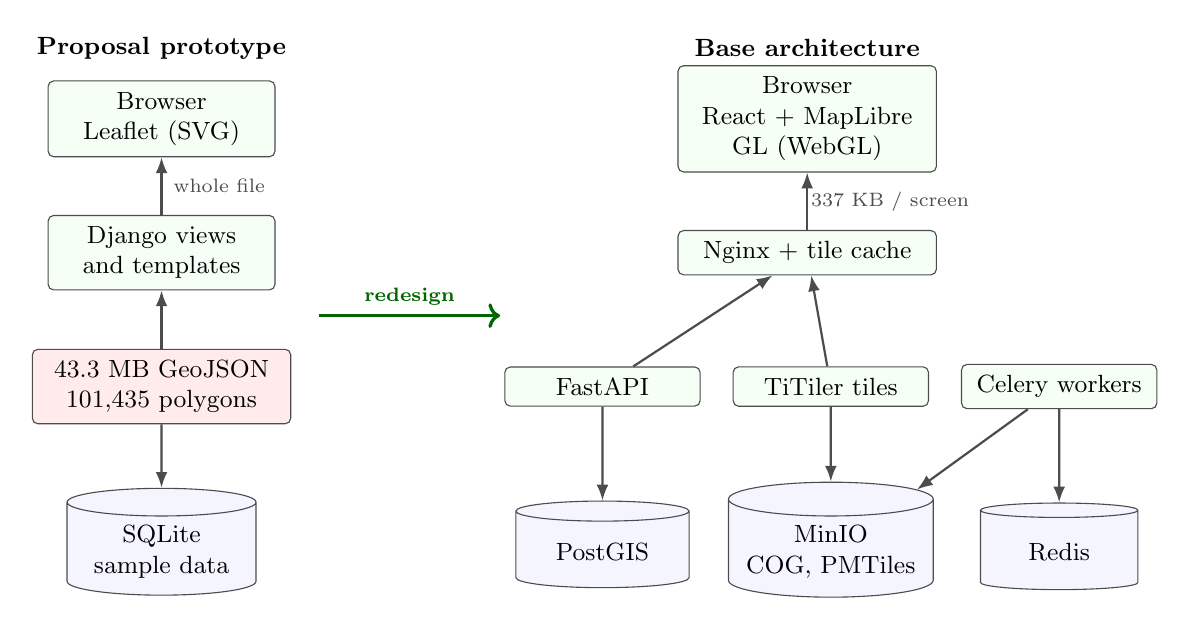
\begin{tikzpicture}[every node/.style={font=\footnotesize}, node distance=0.5cm]
\node[font=\small\bfseries] at (0,0.9) {Proposal prototype};
\node[box, text width=2.6cm] (a1) at (0,0) {Browser\\Leaflet (SVG)};
\node[box, text width=2.6cm] (a2) at (0,-1.7) {Django views and templates};
\node[box, text width=3.0cm, fill=red!8] (a3) at (0,-3.4) {43.3~MB GeoJSON\\101,435 polygons};
\node[dbox, minimum width=2.4cm] (a4) at (0,-5.5) {SQLite\\sample data};
\draw[arr] (a2) -- node[lbl,right=3pt]{whole file} (a1);
\draw[arr] (a3) -- (a2); \draw[arr] (a3) -- (a4);
\node[font=\small\bfseries] at (8.2,0.9) {Base architecture};
\node[box, text width=3.0cm] (b1) at (8.2,0) {Browser\\React + MapLibre GL (WebGL)};
\node[box, text width=3.0cm] (b2) at (8.2,-1.7) {Nginx + tile cache};
\node[box, text width=2.2cm] (b3) at (5.6,-3.4) {FastAPI};
\node[box, text width=2.2cm] (b4) at (8.5,-3.4) {TiTiler tiles};
\node[box, text width=2.2cm] (b5) at (11.4,-3.4) {Celery workers};
\node[dbox, minimum width=2.2cm] (b6) at (5.6,-5.5) {PostGIS};
\node[dbox, minimum width=2.6cm] (b7) at (8.5,-5.5) {MinIO\\COG, PMTiles};
\node[dbox, minimum width=2.0cm] (b8) at (11.4,-5.5) {Redis};
\draw[arr] (b2) -- node[lbl,right]{337~KB / screen} (b1);
\draw[arr] (b3) -- (b2); \draw[arr] (b4) -- (b2);
\draw[arr] (b3) -- (b6); \draw[arr] (b4) -- (b7); \draw[arr] (b5) -- (b8); \draw[arr] (b5) -- (b7);
\draw[->, very thick, green!40!black] (2.0,-2.5) -- node[above, font=\scriptsize\bfseries]{redesign} (4.3,-2.5);
\end{tikzpicture}
\caption{Design evolution: from one large GeoJSON response to tile-based delivery with background processing.}
\end{figure}

\begin{table}[H]
\centering\small
\caption{Design evolution since the proposal}
\label{tab:evolution}
\begin{tabularx}{\textwidth}{L{2.6cm} L{3.6cm} L{4.0cm} Y}
\toprule
\textbf{Aspect} & \textbf{Proposal prototype} & \textbf{Current design} & \textbf{Reason}\\
\midrule
Result format & GeoJSON polygons (43.3~MB) & COG rasters + PMTiles & Data volume and rendering cost\\
Map client & Leaflet, SVG & MapLibre GL, WebGL tiles & Smooth zoom with many layers\\
Backend & Django views and templates & FastAPI + React SPA & Async API, typed contracts, separation of concerns\\
Database & SQLite & PostgreSQL + PostGIS & Spatial queries, concurrency, catalogue\\
Processing & None (upload recorded only) & Celery jobs with progress & Real analysis of new imagery\\
Models & Offline scripts writing GeoJSON & Registry plug-ins writing rasters & Add models without code changes\\
Dashboard data & Hard-coded sample fields & Pre-computed statistics in PostGIS & Real results\\
Deployment & Single process & Seven containers via Compose & Reproducible, scalable services\\
\bottomrule
\end{tabularx}
\end{table}

\section{Architecture Artifacts}
\begin{figure}[H]
\centering
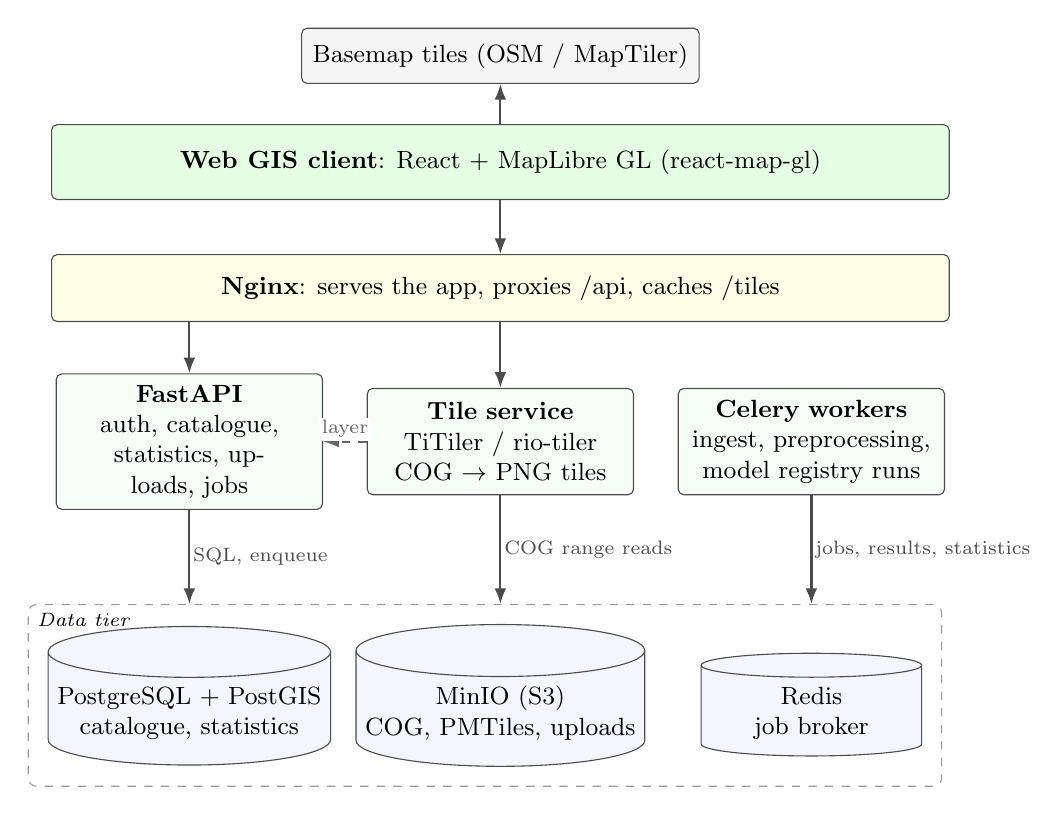
\begin{tikzpicture}[every node/.style={font=\small}]
\node[box, minimum width=4.2cm, minimum height=0.7cm, fill=gray!8] (base) at (0,1.35) {Basemap tiles (OSM / MapTiler)};
\node[box, minimum width=11.4cm, minimum height=0.95cm, fill=green!10] (client) at (0,0) {\textbf{Web GIS client}: React + MapLibre GL (react-map-gl)};
\node[box, minimum width=11.4cm, minimum height=0.85cm, fill=yellow!10] (nginx) at (0,-1.6) {\textbf{Nginx}: serves the app, proxies /api, caches /tiles};
\node[box, text width=3.1cm, minimum height=1.35cm] (api) at (-3.95,-3.55) {\textbf{FastAPI}\\auth, catalogue, statistics, uploads, jobs};
\node[box, text width=3.1cm, minimum height=1.35cm] (tiles) at (0,-3.55) {\textbf{Tile service}\\TiTiler / rio-tiler\\COG $\rightarrow$ PNG tiles};
\node[box, text width=3.1cm, minimum height=1.35cm] (worker) at (3.95,-3.55) {\textbf{Celery workers}\\ingest, preprocessing, model registry runs};
\node[dbox, minimum width=2.8cm] (pg) at (-3.95,-7.0) {PostgreSQL + PostGIS\\catalogue, statistics};
\node[dbox, minimum width=2.8cm] (s3) at (0,-7.0) {MinIO (S3)\\COG, PMTiles, uploads};
\node[dbox, minimum width=2.8cm] (redis) at (3.95,-7.0) {Redis\\job broker};
\node[lane, fit=(pg)(s3)(redis), inner sep=7pt, label={[font=\scriptsize\itshape, anchor=north west]north west:Data tier}] (data) {};
\draw[arr] (client) -- (base);
\draw[arr] (client) -- (nginx);
\draw[arr] (nginx.south -| api.north) -- (api.north);
\draw[arr] (nginx.south -| tiles.north) -- (tiles.north);
\draw[darr] (tiles.west) -- node[lbl,above]{layer} (api.east);
\draw[arr] (api.south) -- node[lbl,right]{SQL, enqueue} (api.south |- data.north);
\draw[arr] (tiles.south) -- node[lbl,right]{COG range reads} (tiles.south |- data.north);
\draw[arr] (worker.south) -- node[lbl,right]{jobs, results, statistics} (worker.south |- data.north);
\end{tikzpicture}
\caption{GeoCrop system architecture. The browser also reads PMTiles and uploads imagery directly to object storage using short-lived signed URLs; the tile service looks up layer styles from the API.}
\label{fig:arch}
\end{figure}

\begin{table}[H]
\centering\small
\caption{Architectural components}
\label{tab:components}
\begin{tabularx}{\textwidth}{L{3.0cm} L{3.4cm} Y}
\toprule
\textbf{Component} & \textbf{Technology} & \textbf{Responsibility}\\
\midrule
Web GIS client & React, Vite, TypeScript, MapLibre GL via react-map-gl, TanStack Query, Zustand & Home, Live Map workspace, Dashboard, Analyze Imagery, Processing, Models, Status, accounts. Builds layers from the catalogue; loads tiles on demand.\\
Edge & Nginx & Serves the built app; proxies the API; caches tiles with immutable headers; resolves services through Docker DNS at request time.\\
API service & FastAPI, Pydantic, SQLAlchemy 2, GeoAlchemy2, PyJWT, bcrypt & REST API v1: health, auth, areas, models, layers, fields, point query, statistics, uploads, runs, jobs.\\
Tile service & TiTiler / rio-tiler (FastAPI) & \code{/tiles/{layer}/{version}/{z}/{x}/{y}.png}; reads only needed COG blocks; applies the server-side style; optional crop filter.\\
Workers & Celery & Ingest (validate, reproject, COG), model runs through the registry, statistics, layer publishing, progress.\\
Model registry & Python package with YAML manifests & Discovers models, resolves dependencies, runs tasks with a common context; built-in cropland, crop type, NDVI index, boundary and yield placeholders.\\
Spatial database & PostgreSQL 16 + PostGIS 3.4, Alembic & Catalogue of users, areas, uploads, images, models, runs, layers, statistics, field regions, jobs.\\
Job broker & Redis 7 & Celery broker and result backend.\\
Object storage & MinIO (S3 API) & Uploads, COG imagery and results, PMTiles; anonymous read only for vector tiles.\\
\bottomrule
\end{tabularx}
\end{table}

\begin{table}[H]
\centering\small
\caption[Main REST interfaces]{Main REST interfaces (prefix \code{/api/v1}; interactive documentation at \code{/api/docs})}
\label{tab:api}
\begin{tabularx}{\textwidth}{L{5.2cm} Y}
\toprule
\textbf{Endpoint} & \textbf{Purpose}\\
\midrule
\code{GET /health} & Status of database, broker, storage, tiles and model registry; configuration notes.\\
\code{POST /auth/signup}, \code{/auth/login}, \code{GET /auth/me} & Accounts and tokens.\\
\code{GET /aois} & Areas visible to the user, with bounds.\\
\code{GET /models} & Registered models, status, inputs, outputs, accuracy and per-class scores.\\
\code{GET /layers?aoi=&kind=&run=} & Layer catalogue: style, legend, bounds, zoom range, tile URL, version.\\
\code{GET /fields?aoi=&q=} & Field regions with crop, area and bounding box.\\
\code{GET /point?lng=&lat=&layers=} & Values and labels of several layers at one location.\\
\code{GET /stats?layer=} & Pre-computed area and share per class.\\
\code{POST /uploads}, \code{/uploads/{id}/complete} & Signed upload URL; start ingestion with models, location and date.\\
\code{POST /runs}, \code{GET /runs}, \code{GET /jobs/{id}} & Re-run models; run history; job progress and steps.\\
\code{GET /tiles/{layer}/{v}/{z}/{x}/{y}.png} & Raster tiles (tile service, cached by Nginx).\\
\bottomrule
\end{tabularx}
\end{table}

\begin{table}[H]
\centering\small
\caption{Key architecture decisions}
\label{tab:adr}
\begin{tabularx}{\textwidth}{L{3.6cm} Y L{3.6cm}}
\toprule
\textbf{Decision} & \textbf{Rationale} & \textbf{Alternative rejected}\\
\midrule
Raster as source of truth (COG) & Models predict pixels; a 30~m raster of AOI1 is about 1.6~MB, the same result as polygons 43.3~MB. & Vectorising all output to GeoJSON\\
Tiles via TiTiler & Reads only the COG blocks needed per tile; styles applied on the server; no pre-rendering. & Pre-rendered tile folders; single PNG overlays\\
PMTiles for vectors & One static file read by range requests; no tile server; cacheable. & GeoJSON; dynamic vector tile server\\
MapLibre GL & WebGL rendering of raster and vector tiles; open source. & Leaflet (SVG/Canvas)\\
Versioned, immutable tile URLs & Browsers and Nginx can cache for a year; a new run gets a new URL. & Cache invalidation logic\\
FastAPI & Same stack as TiTiler; async I/O; typed schemas and generated docs. & Django templates (prototype)\\
PostgreSQL + PostGIS & Spatial types and indexes, joins between catalogue and statistics, JSONB for styles and metrics. & SQLite (prototype)\\
Celery + Redis & Long jobs off the request path; retries; progress. & Synchronous processing\\
S3-compatible storage (MinIO) & Large files, range reads, signed uploads, cloud-portable. & Local disk\\
Manifest-based model registry & Models change over the project; new models without changes elsewhere. & Hard-coded model calls\\
Docker Compose & One-command, reproducible stack for the team and the panel. & Manual installation\\
\bottomrule
\end{tabularx}
\end{table}

\section{Requirements and Domain Artifacts}
\begin{figure}[H]
\centering
\resizebox{\textwidth}{!}{%
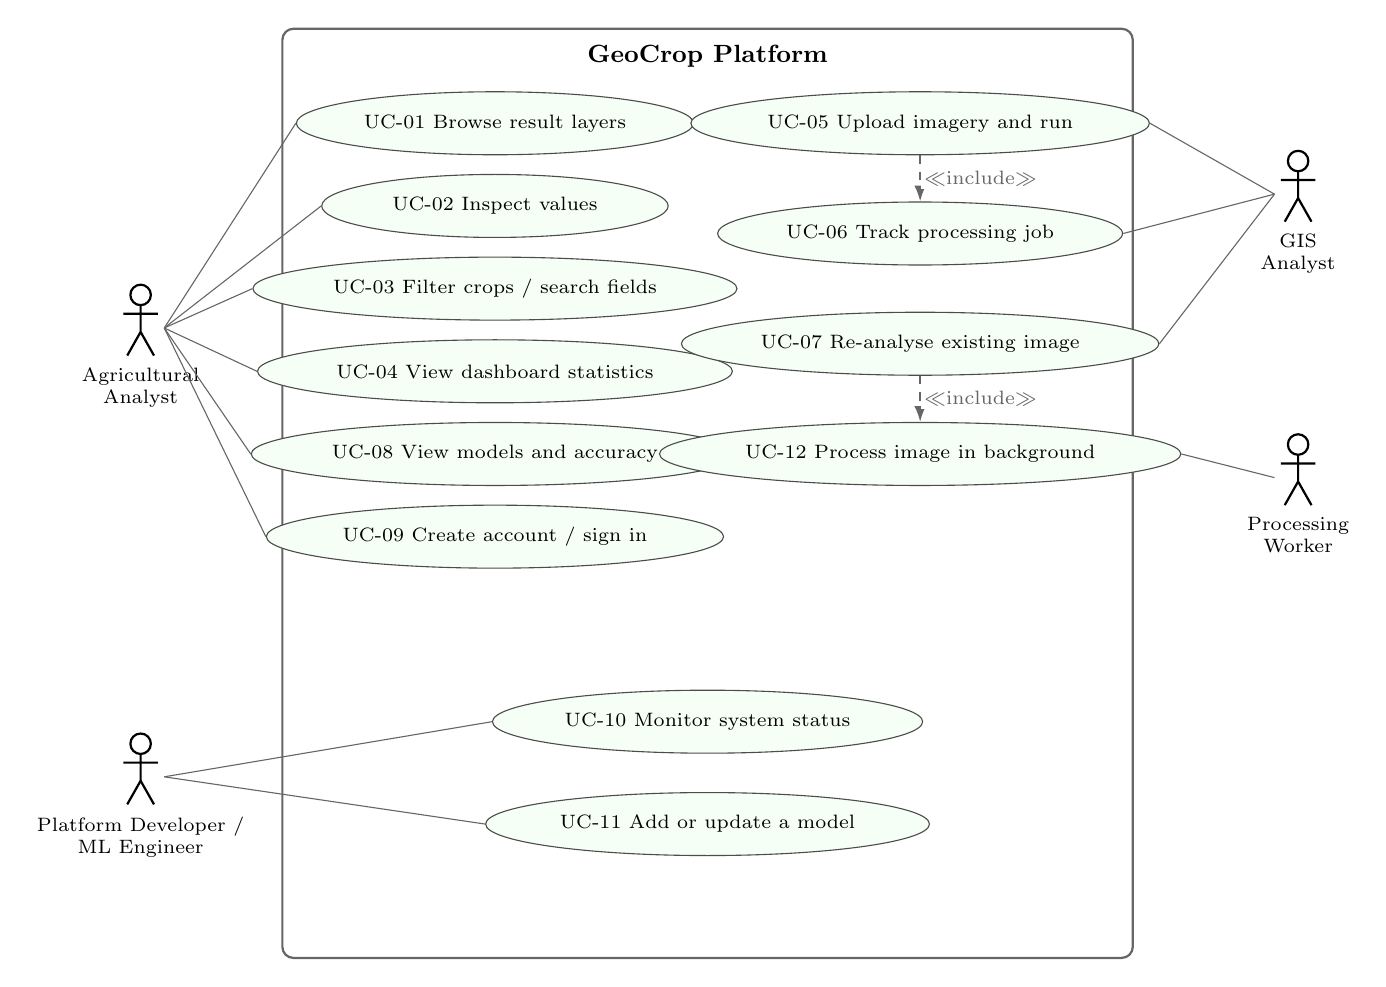
\begin{tikzpicture}[
  uc/.style={draw=black!70, ellipse, fill=green!4, minimum width=4.4cm, minimum height=0.8cm, font=\scriptsize, align=center},
  actor/.style={font=\scriptsize, align=center}]
\newcommand{\stick}[2]{%
  \begin{scope}[shift={(#1)}]
  \draw[thick] (0,0.42) circle (0.13);
  \draw[thick] (0,0.29) -- (0,-0.05) (-0.22,0.18) -- (0.22,0.18) (0,-0.05) -- (-0.17,-0.35) (0,-0.05) -- (0.17,-0.35);
  \node[actor, below] at (0,-0.38) {#2};
  \end{scope}}
\draw[rounded corners=4pt, thick, black!60] (-2.7,-6.3) rectangle (8.1,5.5);
\node[font=\small\bfseries] at (2.7,5.15) {GeoCrop Platform};
\node[uc] (u1) at (0,4.3) {UC-01 Browse result layers};
\node[uc] (u2) at (0,3.25) {UC-02 Inspect values};
\node[uc] (u3) at (0,2.2) {UC-03 Filter crops / search fields};
\node[uc] (u4) at (0,1.15) {UC-04 View dashboard statistics};
\node[uc] (u8) at (0,0.1) {UC-08 View models and accuracy};
\node[uc] (u9) at (0,-0.95) {UC-09 Create account / sign in};
\node[uc] (u5) at (5.4,4.3) {UC-05 Upload imagery and run};
\node[uc] (u6) at (5.4,2.9) {UC-06 Track processing job};
\node[uc] (u7) at (5.4,1.5) {UC-07 Re-analyse existing image};
\node[uc] (u12) at (5.4,0.1) {UC-12 Process image in background};
\node[uc] (u10) at (2.7,-3.3) {UC-10 Monitor system status};
\node[uc] (u11) at (2.7,-4.6) {UC-11 Add or update a model};
\stick{-4.5,1.7}{Agricultural\\Analyst}
\stick{10.2,3.4}{GIS\\Analyst}
\stick{-4.5,-4.0}{Platform Developer /\\ML Engineer}
\stick{10.2,-0.2}{Processing\\Worker}
\foreach \u in {u1,u2,u3,u4,u8,u9} \draw[black!60] (-4.2,1.7) -- (\u.west);
\foreach \u in {u5,u6,u7} \draw[black!60] (9.9,3.4) -- (\u.east);
\draw[black!60] (9.9,-0.2) -- (u12.east);
\draw[black!60] (-4.2,-4.0) -- (u10.west);
\draw[black!60] (-4.2,-4.0) -- (u11.west);
\draw[darr] (u5.south) -- node[lbl, right] {$\ll$include$\gg$} (u6.north);
\draw[darr] (u7.south) -- node[lbl, right] {$\ll$include$\gg$} (u12.north);
\end{tikzpicture}}
\caption{Use case diagram of the GeoCrop platform}
\label{fig:usecase}
\end{figure}

\begin{figure}[H]
\centering
\resizebox{\textwidth}{!}{%
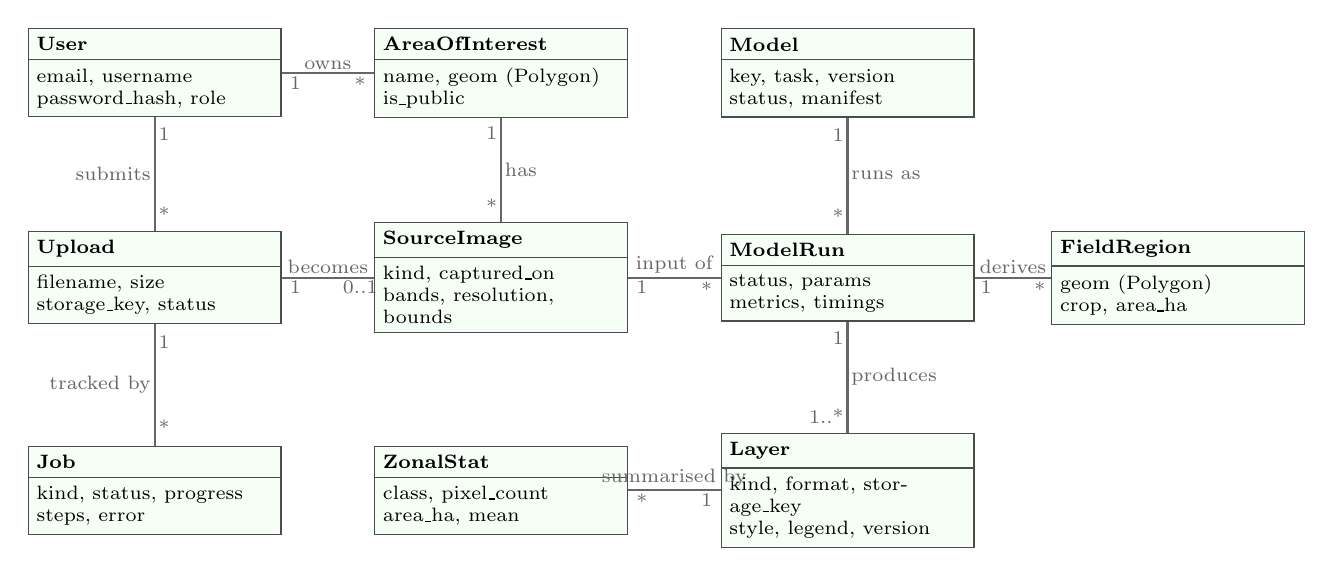
\begin{tikzpicture}[
  cls/.style={draw=black!70, rectangle split, rectangle split parts=2, fill=green!4, font=\scriptsize, align=left, text width=3.0cm, inner sep=3pt, rectangle split part fill={green!14,green!3}},
  rel/.style={thick, black!60}, m/.style={font=\scriptsize, inner sep=1pt}]
\node[cls] (user) at (0,0) {\textbf{User}\nodepart{second}email, username\\password\_hash, role};
\node[cls] (aoi) at (4.4,0) {\textbf{AreaOfInterest}\nodepart{second}name, geom (Polygon)\\is\_public};
\node[cls] (upload) at (0,-2.6) {\textbf{Upload}\nodepart{second}filename, size\\storage\_key, status};
\node[cls] (img) at (4.4,-2.6) {\textbf{SourceImage}\nodepart{second}kind, captured\_on\\bands, resolution, bounds};
\node[cls] (model) at (8.8,0) {\textbf{Model}\nodepart{second}key, task, version\\status, manifest};
\node[cls] (run) at (8.8,-2.6) {\textbf{ModelRun}\nodepart{second}status, params\\metrics, timings};
\node[cls] (layer) at (8.8,-5.3) {\textbf{Layer}\nodepart{second}kind, format, storage\_key\\style, legend, version};
\node[cls] (stat) at (4.4,-5.3) {\textbf{ZonalStat}\nodepart{second}class, pixel\_count\\area\_ha, mean};
\node[cls] (field) at (13.0,-2.6) {\textbf{FieldRegion}\nodepart{second}geom (Polygon)\\crop, area\_ha};
\node[cls] (job) at (0,-5.3) {\textbf{Job}\nodepart{second}kind, status, progress\\steps, error};
\draw[rel] (user) -- node[m,above]{owns} node[m,pos=0.15,below]{1} node[m,pos=0.85,below]{*} (aoi);
\draw[rel] (user) -- node[m,left]{submits} node[m,pos=0.15,right]{1} node[m,pos=0.85,right]{*} (upload);
\draw[rel] (upload) -- node[m,above]{becomes} node[m,pos=0.15,below]{1} node[m,pos=0.85,below]{0..1} (img);
\draw[rel] (aoi) -- node[m,right]{has} node[m,pos=0.15,left]{1} node[m,pos=0.85,left]{*} (img);
\draw[rel] (model) -- node[m,right]{runs as} node[m,pos=0.15,left]{1} node[m,pos=0.85,left]{*} (run);
\draw[rel] (img) -- node[m,above]{input of} node[m,pos=0.15,below]{1} node[m,pos=0.85,below]{*} (run);
\draw[rel] (run) -- node[m,right]{produces} node[m,pos=0.15,left]{1} node[m,pos=0.85,left]{1..*} (layer);
\draw[rel] (layer) -- node[m,above]{summarised by} node[m,pos=0.15,below]{1} node[m,pos=0.85,below]{*} (stat);
\draw[rel] (run) -- node[m,above]{derives} node[m,pos=0.15,below]{1} node[m,pos=0.85,below]{*} (field);
\draw[rel] (upload) -- node[m,left]{tracked by} node[m,pos=0.15,right]{1} node[m,pos=0.85,right]{*} (job);
\end{tikzpicture}}
\caption{Domain model}
\label{fig:domain}
\end{figure}

\section{Data Design}
\begin{table}[H]
\centering\small
\caption{Database tables}
\label{tab:schema}
\begin{tabularx}{\textwidth}{L{2.4cm} Y}
\toprule
\textbf{Table} & \textbf{Key columns}\\
\midrule
\code{users} & id, email (unique), username (unique), password\_hash, role, created\_at\\
\code{aoi} & id, owner\_id, name, geom (Polygon, GiST), is\_public\\
\code{upload} & id, user\_id, aoi\_id, filename, size\_bytes, storage\_key, status\\
\code{source_image} & id, aoi\_id, upload\_id, kind, captured\_on, storage\_key, bounds (GiST), band\_count, resolution\_m\\
\code{model} & id, key (unique), task, version, name, status, manifest (JSONB), enabled\\
\code{model_run} & id, aoi\_id, model\_id, source\_image\_id, status, params, metrics (JSONB), error, timings\\
\code{map_layer} & id, run\_id, aoi\_id, kind, group, name, format, storage\_key, bounds (GiST), zoom range, nodata, style, legend (JSONB), version, is\_public\\
\code{zonal_stat} & layer\_id, zone\_type, zone\_id, class\_code, class\_name, pixel\_count, area\_ha, mean, min, max\\
\code{field} & id, aoi\_id, run\_id, geom (Polygon, GiST), attributes (JSONB)\\
\code{job} & id, kind, status, progress, message, error, steps (JSONB), upload\_id, user\_id\\
\bottomrule
\end{tabularx}
\end{table}

\section{Behaviour and Deployment Artifacts}
\begin{figure}[H]
\centering
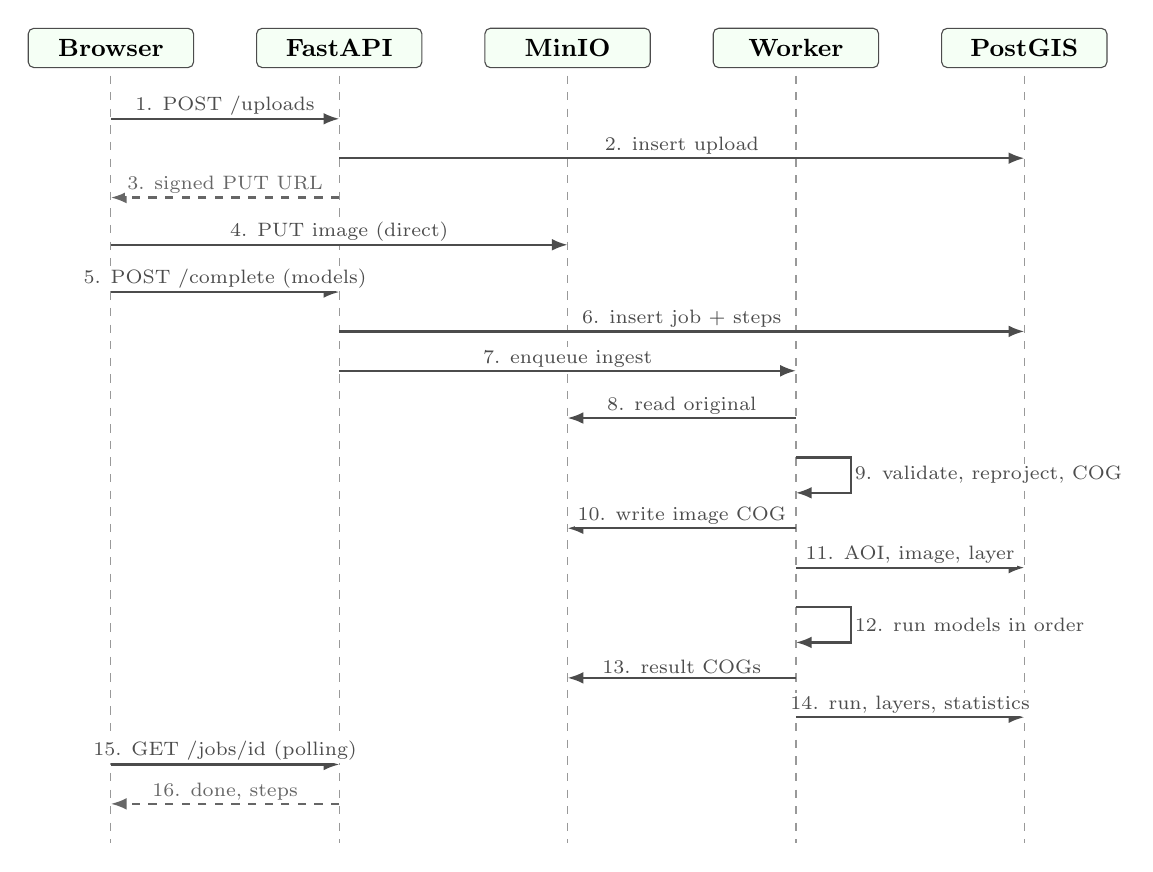
\begin{tikzpicture}[font=\scriptsize]
\foreach \x/\n/\t in {0/b/Browser, 2.9/a/FastAPI, 5.8/s/MinIO, 8.7/w/Worker, 11.6/d/PostGIS}{
  \node[box, minimum width=2.1cm] (\n) at (\x,0) {\textbf{\t}};
  \draw[dashed, black!40] (\x,-0.35) -- (\x,-10.1);
}
\newcommand{\msg}[5]{\draw[#5] (#1,#3) -- node[lbl,above]{#4} (#2,#3);}
\msg{0}{2.9}{-0.9}{1. POST /uploads}{arr}
\msg{2.9}{11.6}{-1.4}{2. insert upload}{arr}
\msg{2.9}{0}{-1.9}{3. signed PUT URL}{darr}
\msg{0}{5.8}{-2.5}{4. PUT image (direct)}{arr}
\msg{0}{2.9}{-3.1}{5. POST /complete (models)}{arr}
\msg{2.9}{11.6}{-3.6}{6. insert job + steps}{arr}
\msg{2.9}{8.7}{-4.1}{7. enqueue ingest}{arr}
\msg{8.7}{5.8}{-4.7}{8. read original}{arr}
\draw[arr] (8.7,-5.2) -- ++(0.7,0) -- node[lbl,right]{9. validate, reproject, COG} ++(0,-0.45) -- ++(-0.7,0);
\msg{8.7}{5.8}{-6.1}{10. write image COG}{arr}
\msg{8.7}{11.6}{-6.6}{11. AOI, image, layer}{arr}
\draw[arr] (8.7,-7.1) -- ++(0.7,0) -- node[lbl,right]{12. run models in order} ++(0,-0.45) -- ++(-0.7,0);
\msg{8.7}{5.8}{-8.0}{13. result COGs}{arr}
\msg{8.7}{11.6}{-8.5}{14. run, layers, statistics}{arr}
\msg{0}{2.9}{-9.1}{15. GET /jobs/{id} (polling)}{arr}
\msg{2.9}{0}{-9.6}{16. done, steps}{darr}
\end{tikzpicture}
\caption{Sequence of an upload and analysis}
\label{fig:seq}
\end{figure}

\begin{figure}[H]
\centering
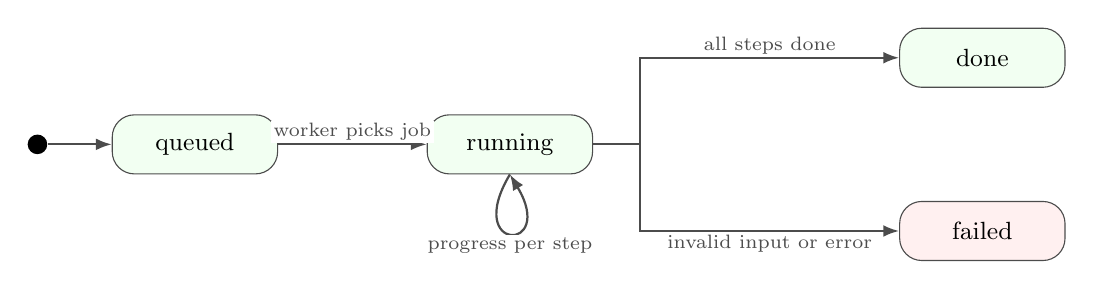
\begin{tikzpicture}[st/.style={draw=black!70, rounded corners=8pt, fill=green!5, minimum width=2.1cm, minimum height=0.75cm, font=\small}]
\node[circle, fill=black, inner sep=2.5pt] (start) at (0,0) {};
\node[st] (q) at (2,0) {queued};
\node[st] (r) at (6,0) {running};
\node[st] (d) at (12,1.1) {done};
\node[st, fill=red!6] (f) at (12,-1.1) {failed};
\draw[arr] (start) -- (q);
\draw[arr] (q) -- node[lbl,above]{worker picks job} (r);
\draw[arr] (r.east) -- ++(0.6,0) |- node[lbl,pos=0.75,above]{all steps done} (d.west);
\draw[arr] (r.east) -- ++(0.6,0) |- node[lbl,pos=0.75,below]{invalid input or error} (f.west);
\draw[arr] (r.south) .. controls +(-0.6,-1.0) and +(0.6,-1.0) .. node[lbl,below]{progress per step} (r.south);
\end{tikzpicture}
\caption{Job state machine}
\label{fig:states}
\end{figure}

\begin{figure}[H]
\centering
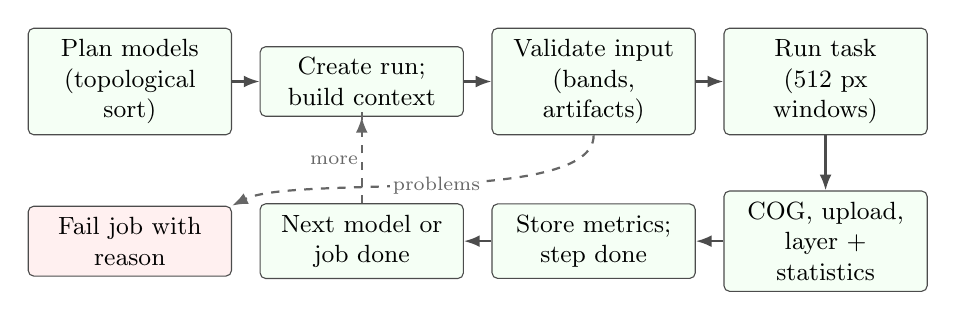
\begin{tikzpicture}[node distance=0.35cm, every node/.style={font=\scriptsize}]
\node[box, text width=2.3cm] (p1) {Plan models\\(topological sort)};
\node[box, text width=2.3cm, right=of p1] (p2) {Create run;\\build context};
\node[box, text width=2.3cm, right=of p2] (p3) {Validate input\\(bands, artifacts)};
\node[box, text width=2.3cm, right=of p3] (p4) {Run task\\(512 px windows)};
\node[box, text width=2.3cm, below=0.7cm of p4] (p5) {COG, upload,\\layer + statistics};
\node[box, text width=2.3cm, left=of p5] (p6) {Store metrics;\\step done};
\node[box, text width=2.3cm, left=of p6] (p7) {Next model or\\job done};
\node[box, text width=2.3cm, left=of p7, fill=red!6] (p8) {Fail job with\\reason};
\draw[arr] (p1)--(p2); \draw[arr] (p2)--(p3); \draw[arr] (p3)--(p4); \draw[arr] (p4)--(p5);
\draw[arr] (p5)--(p6); \draw[arr] (p6)--(p7);
\draw[darr] (p3.south) .. controls +(0,-0.9) and +(0.8,0.4) .. node[lbl,pos=0.5]{problems} (p8.north east);
\draw[darr] (p7.north) -- node[lbl,left]{more} (p7.north |- p2.south) -- (p2.south);
\end{tikzpicture}
\caption{Activity of a model run inside the worker}
\label{fig:activity}
\end{figure}

\begin{figure}[H]
\centering
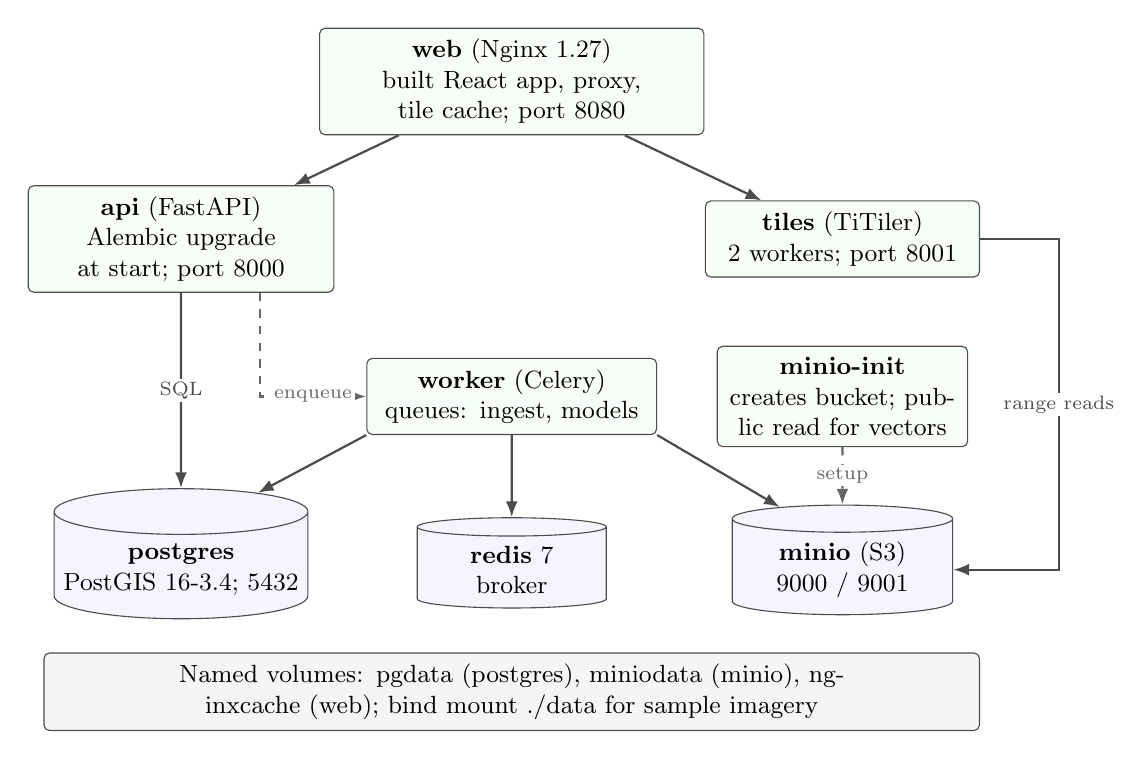
\begin{tikzpicture}[every node/.style={font=\scriptsize}]
\node[box, text width=4.6cm] (web) at (0,0) {\textbf{web} (Nginx 1.27)\\built React app, proxy, tile cache; port 8080};
\node[box, text width=3.6cm] (api) at (-4.2,-2.0) {\textbf{api} (FastAPI)\\Alembic upgrade at start; port 8000};
\node[box, text width=3.2cm] (tiles) at (4.2,-2.0) {\textbf{tiles} (TiTiler)\\2 workers; port 8001};
\node[box, text width=3.4cm] (worker) at (0,-4.0) {\textbf{worker} (Celery)\\queues: ingest, models};
\node[box, text width=2.9cm] (init) at (4.2,-4.0) {\textbf{minio-init}\\creates bucket; public read for vectors};
\node[dbox, minimum width=3.0cm] (pg) at (-4.2,-6.2) {\textbf{postgres}\\PostGIS 16-3.4; 5432};
\node[dbox, minimum width=2.4cm] (redis) at (0,-6.2) {\textbf{redis} 7\\broker};
\node[dbox, minimum width=2.8cm] (minio) at (4.2,-6.2) {\textbf{minio} (S3)\\9000 / 9001};
\node[box, text width=11.6cm, fill=gray!8] (vol) at (0,-7.75) {Named volumes: pgdata (postgres), miniodata (minio), nginxcache (web); bind mount ./data for sample imagery};
\draw[arr] (web) -- (api); \draw[arr] (web) -- (tiles);
\draw[arr] (api) -- node[lbl]{SQL} (pg);
\draw[darr] (api.south) ++(1.0,0) |- node[lbl,pos=0.75]{enqueue} (worker.west);
\draw[arr] (worker) -- (redis);
\draw[arr] (worker.south west) -- (pg.north east);
\draw[arr] (worker.south east) -- (minio.north west);
\draw[arr] (tiles.east) -- ++(1.0,0) |- node[lbl,pos=0.25]{range reads} (minio.east);
\draw[darr] (init) -- node[lbl]{setup} (minio);
\end{tikzpicture}
\caption{Deployment view of the Docker Compose stack}
\label{fig:deploy}
\end{figure}
\end{document}
